\documentclass[12pt]{article}
\usepackage{ulem}
\usepackage{float}
\usepackage{mhchem}
\usepackage{pdfpages}
\usepackage{enumerate}
\usepackage{amsmath}
\usepackage{amssymb}
\usepackage{graphicx}
\usepackage{subfigure}
\usepackage{leftidx}
\usepackage{geometry}
\usepackage{wrapfig}
\usepackage{extarrows}
\usepackage{url}
\usepackage{multirow}

\renewcommand\thesection{\Roman{section}}
\renewcommand\thesubsection{\Alph{subsection}}
\geometry{a4paper,left=2.54cm,right=2.54cm,top=2.54cm,bottom=2.54cm}
\begin{document}

\section{Coutte Flow}

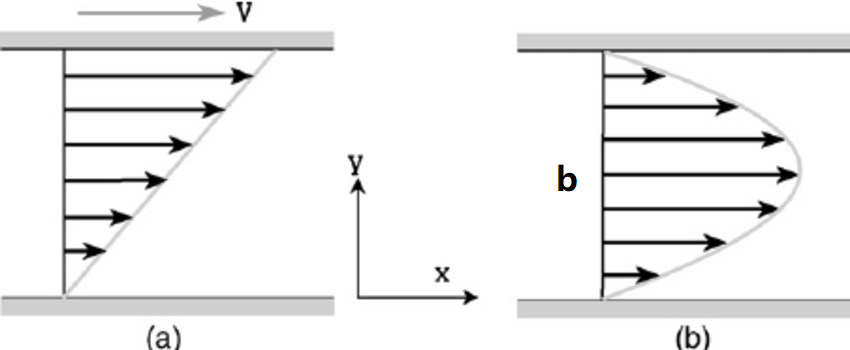
\includegraphics[width=\textwidth]{coutte_flow.png}

The general formula should be
\begin{equation}
    u = \frac{1}{2\mu} (\frac{\partial P}{\partial x}) y^2 + C_1y + C_2
\end{equation}
where $C_1$ and $C_2$ are constants.

Consider the boundary conditions:
\begin{itemize}
    \item $u$ = 0 at $y$ = 0; $u$=$U$ at $y=b$:
        $$ u = U\frac{y}{b} + \frac{1}{2\mu}(\frac{\partial P}{\partial x})(y^2 - by) $$
    \item $u=U$ at both $y=0$ and $y=b$:
        $$  u = U + \frac{1}{2\mu}(\frac{\partial P}{\partial x})(y^2 - by) $$
\end{itemize}

Since the shear force is calculated through $\tau = \mu \frac{\mathrm{d}u}{\mathrm{d}y}$,
then the shear stresses can be calculated as follows (\textbf{boundary conditions: $u = u_1$ at $y=0$; $u = u_2$ at $y = b$}):
$$ \tau(y) = (\frac{\partial P}{\partial x})(y - \frac{b}{2}) + \mu \frac{u_2 - u_1}{b} $$

Special cases:
\begin{itemize}
    \item $u$ = 0 at $y$ = 0; $u$=$U$ at $y=b$:
        $$ \tau = \mu \frac{U}{b} + \frac{1}{2}(\frac{\partial P}{\partial x})b $$
    \item $u=U$ at both $y=0$ and $y=b$:
        $$  \tau =  \frac{1}{2}(\frac{\partial P}{\partial x})b $$
\end{itemize}




\end{document}